\Large\textbf{}\\
\Large\textbf{Use Case 6 Creazione Oggetto} \\
\vspace{0.5cm}
\begin{figure}[h]
 \centering
 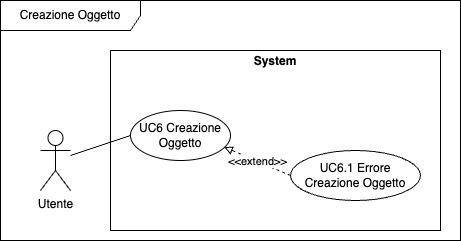
\includegraphics[width=0.8\textwidth]{UseCasesImages/ObjCreation.png}
\end{figure}

\large\textbf{} \\
\textbf{Attori:} User\\
\textbf{Pre-condizione:} Magazzino correttamente istanziato \\
\textbf{Post-condizione: } Creazione di un oggetto\\
\textbf{Scenario Principale:}\\
\begin{itemize}
  \item L'utente inserisce un codice identificativo dell'oggetto
  \item L'oggetto viene creato
\end{itemize}.\\
\textbf{Estensioni: } UC6.1 Errore Creazione Oggetto\\

\vspace{0.5cm}

{\color{red}{\textbf{Domanda:} La creazione di un oggetto puó avvenire anche senza inserimento?}}

\vspace{0.5cm}

\Large\textbf{}\\
\Large\textbf{Use Case 6.1 Errore Creazione Oggetto} \\
\large\textbf{} \\
\textbf{Attori:} User\\
\textbf{Pre-condizione:} L'utente ha inserito dati scorretti nella schermata di creazione di un oggetto\\
\textbf{Post-condizione: } Visualizzazione Errore\\
\textbf{Scenario Principale:} Il sistema mostra a schermo un messaggio contenente le specifiche dell'errore di inserimento\\

\vspace{0.5cm}

\Large\textbf{}\\
\Large\textbf{Use Case 7 Ricerca Oggetto tramite Id} \\
\vspace{0.5cm}
\begin{figure}[h]
  \centering
  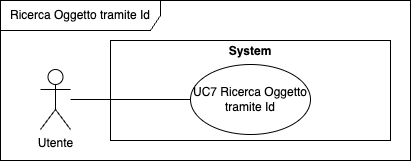
\includegraphics[width=0.8\textwidth]{UseCasesImages/ObjResearchId.drawio.png}
\end{figure}

\large\textbf{} \\
\textbf{Attori:} User\\
\textbf{Pre-condizione:}  Magazzino correttamente istanziato\\
\textbf{Post-condizione: } Visualizzazione risultato ricerca\\
\textbf{Scenario Principale:} \\
\begin{itemize}
  \item L'utente immette un codice identificativo
  \item Il sistema visualizza l'oggetto corrispondente, se trovato, oppure comunica l'assenza di un risultato
\end{itemize}.

\vspace{0.5cm}

\Large\textbf{}\\
\Large\textbf{Use Case 8 Selezione Oggetto} \\
\begin{figure}[h]
  \centering
 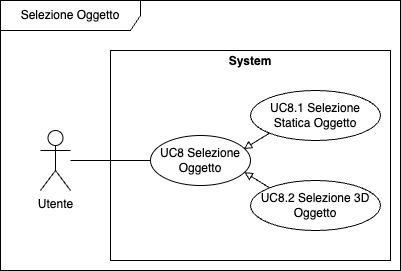
\includegraphics[width=0.8\textwidth]{UseCasesImages/ObjSelection.drawio.png}
\end{figure}

\vspace{0.5cm}

\large\textbf{} \\
\textbf{Attori:} User\\
\textbf{Pre-condizione:} Sistema correttamente istanziato \\
\textbf{Post-condizione: } Selezione di un oggetto\\
\textbf{Scenario Principale:}  
 L'utente seleziona un oggetto attraverso [UC9] o [UC10]
\textbf{Generalizzazioni:} 
\begin{itemize}
    \item UC9 Selezione Statica Oggetto
    \item UC10 Selezione 3D Oggetto
\end{itemize}

\Large\textbf{}\\
\Large\textbf{Use Case 8.1 Selezione Statica Oggetto} \\
%\begin{figure}[h]
%  \centering
%  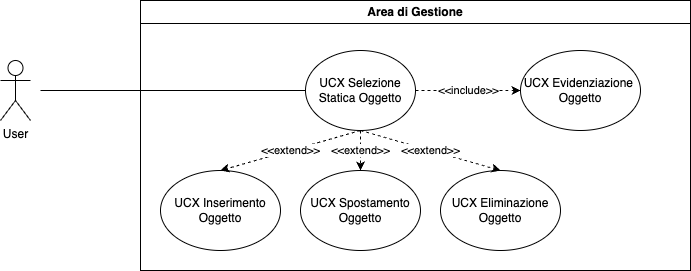
\includegraphics[width=0.8\textwidth]{UseCasesImages/StaticSel.png}
%\end{figure}

\vspace{0.5cm}

\large\textbf{} \\
\textbf{Attori:} User\\
\textbf{Pre-condizione:} L'utente ha effettuato [UC7] con risultato non nullo \\
\textbf{Post-condizione: }  Selezione di un oggetto con conseguente evidenziazione delle correnti posizioni nell'ambiente tridimensionale\\
\textbf{Scenario Principale:}
\begin{itemize}
    \item L'utente seleziona un oggetto
    \item L'oggetto viene evidenziato nell'ambiente 3D ove presente
\end{itemize}

\vspace{0.5cm}

\Large\textbf{}\\
\Large\textbf{Use Case 8.2 Selezione 3D Oggetto} \\
%\begin{figure}[h]
%  \centering
%  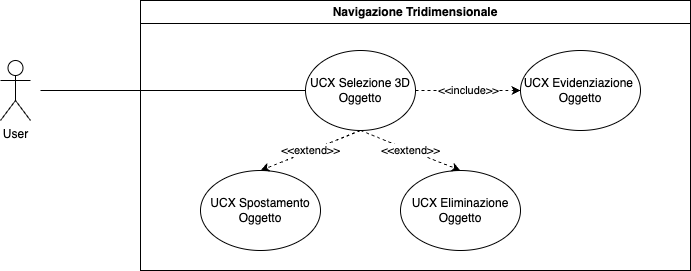
\includegraphics[width=0.8\textwidth]{UseCasesImages/3DSel.png}
%\end{figure}

\large\textbf{} \\
\textbf{Attori:} User\\
\textbf{Pre-condizione:} Sistema correttamente istanziato \\
\textbf{Post-condizione: } Selezione di un oggetto\\
\textbf{Scenario Principale:}
Attraverso la navigazione nello spazio tridimensionale l'utente seleziona un oggetto

\vspace{0.5cm}


\Large\textbf{}\\
\Large\textbf{Use Case 9 Inserimento Oggetto} \\
\begin{figure}[h]
 \centering
  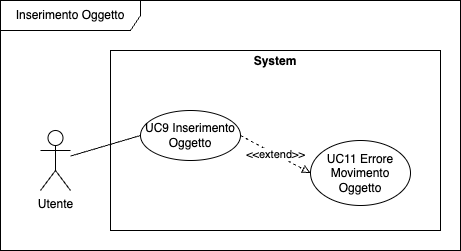
\includegraphics[width=0.8\textwidth]{UseCasesImages/ObjInsert.drawio.png}
\end{figure}

\vspace{0.5cm}

\large\textbf{} \\
\textbf{Attori:} User\\
\textbf{Pre-condizione:} L'utente ha creato ([UC6]) o selezionato ([UC7] un oggetto non ancora inserito  \\
\textbf{Post-condizione: } L'oggetto é stato correttamente inserito o viene visualizzato un messaggio di errore\\
\textbf{Scenario Principale:} 
\begin{itemize}
    \item L'utente seleziona la scaffalatura dove vuole inserire l'oggetto 
    \item Il sistema verifica la disponibilitá della scaffalatura
    \item L'oggetto viene inserito o l'inserimento viene rifiutato con conseguente schermata di errore
\end{itemize}
\textbf{Estensione} UC11 Errore Movimento Oggetto


\large\textbf{} \\
\textbf{Attori:} User\\
\textbf{Pre-condizione:} L'utente sta creando un oggetto \\
\textbf{Post-condizione: } L'utente ha inserito l'id di un oggetto\\
\textbf{Scenario Principale:}\\
\begin{itemize}
  \item L'utente inserisce un codice identificativo dell'oggetto
  \item L'oggetto viene creato
\end{itemize}.\\
\textbf{Estensioni: } UC6.1 Errore Creazione Oggetto\\

\vspace{0.5cm}


\vspace{0.5cm}

\Large\textbf{}\\
\Large\textbf{Use Case 10 Spostamento Oggetto} \\
\begin{figure}[h]
 \centering
 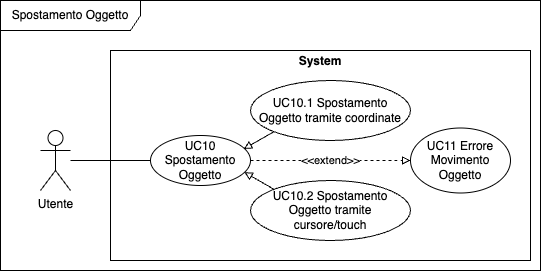
\includegraphics[width=0.8\textwidth]{UseCasesImages/ObjMovement.drawio.png}
\end{figure}

\vspace{0.5cm}

\large\textbf{} \\
\textbf{Attori:} User\\
\textbf{Pre-condizione:} L'utente ha selezionato un oggetto \\
\textbf{Post-condizione: } L'oggetto é stato correttamente spostato o viene visualizzato un messaggio di errore\\
\textbf{Scenario Principale:} 
\begin{itemize}
    \item L'utente sposta l'oggetto mediante [UC10.1] o [UC10.2]
    \item Il sistema verifica la disponibilitá della scaffalatura
    \item L'oggetto viene spostato o il movimento viene rifiutato con conseguente schermata di errore
\end{itemize}
\textbf{Generalizzazioni:}
\begin{itemize}
    \item UC10.1 Spostamento Oggetto tramite coordinate
    \item UC10.2 Spostamento Oggetto tramite cursore/touch
\end{itemize}
\textbf{Estensione} UC11 Errore Movimento Oggetto

\vspace{0.5cm}

\Large\textbf{}\\
\Large\textbf{Use Case 10.1 Spostamento Oggetto tramite coordinate} \\
%\begin{figure}[h]
%  \centering
%  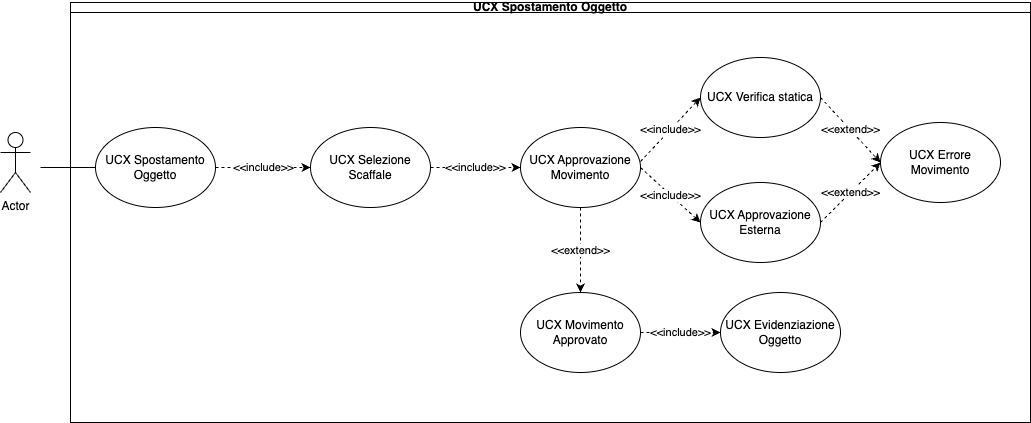
\includegraphics[width=0.8\textwidth]{UseCasesImages/Spostamento.png}
%\end{figure}

\vspace{0.5cm}

\large\textbf{} \\
\textbf{Attori:} User\\
\textbf{Pre-condizione:} L'utente ha selezionato un oggetto \\
\textbf{Post-condizione: } L'oggetto é stato correttamente spostato o viene visualizzato un messaggio di errore\\
\textbf{Scenario Principale:} 
\begin{itemize}
    \item L'utente inserisce le coordinate della scaffalatura in cui vuole spostare l'oggetto
    \item Il sistema verifica la disponibilitá della scaffalatura
    \item L'oggetto viene spostato o il movimento viene rifiutato con conseguente schermata di errore
\end{itemize}

\vspace{0.5cm}

\Large\textbf{}\\
\Large\textbf{Use Case 10.2 Spostamento Oggetto tramite cursore/touch} \\
%\begin{figure}[h]
%  \centering
%  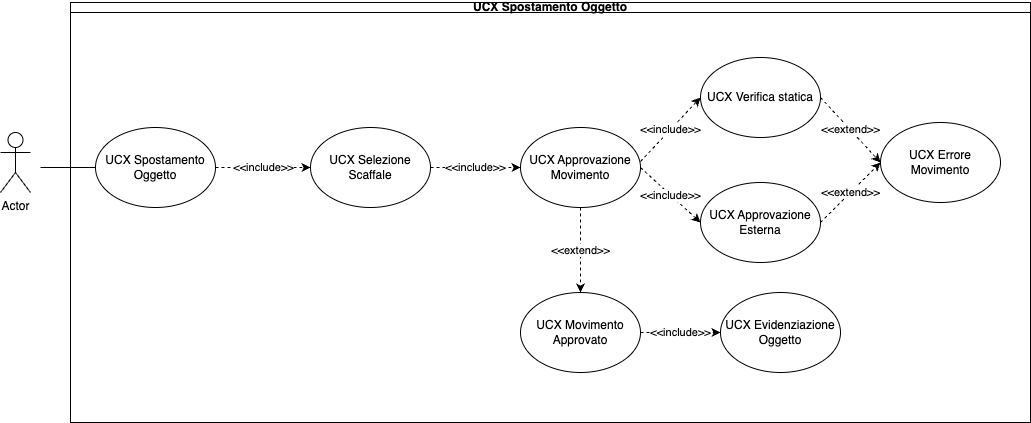
\includegraphics[width=0.8\textwidth]{UseCasesImages/Spostamento.png}
%\end{figure}

\vspace{0.5cm}

\large\textbf{} \\
\textbf{Attori:} User\\
\textbf{Pre-condizione:} L'utente ha selezionato un oggetto \\
\textbf{Post-condizione: } L'oggetto é stato correttamente spostato o viene visualizzato un messaggio di errore\\
\textbf{Scenario Principale:} 
\begin{itemize}
    \item L'utente trascina tramite cursore/touch l'oggetto verso la scaffalatua in cui lo vuole spostare
    \item Il sistema verifica la disponibilitá della scaffalatura
    \item L'oggetto viene spostato o il movimento viene rifiutato con conseguente schermata di errore
\end{itemize}

\vspace{0.5cm}

\Large\textbf{}\\
\Large\textbf{Use Case 11 Errore Movimento Oggetto} \\

\vspace{0.5cm}

\large\textbf{} \\
\textbf{Attori:} Sistema\\
\textbf{Pre-condizione:} L'utente ha richiesto un movimento non possibile di un oggetto  \\
\textbf{Post-condizione: } Viene visualizzato un messaggio di errore\\
\textbf{Scenario Principale:} 
Il sistema visualizza un errore conseguente alla richiesta di un movimento non possibile di un oggetto

\vspace{0.5cm}

\Large\textbf{}\\
\Large\textbf{Use Case 12 Eliminazione Oggetto} \\
\begin{figure}[h]
  \centering
  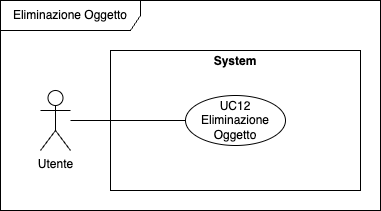
\includegraphics[width=0.8\textwidth]{UseCasesImages/ObjDelete.drawio.png}
\end{figure}
\vspace{0.5cm}

\large\textbf{} \\
\textbf{Attori:} User\\
\textbf{Pre-condizione:} L'utente ha selezionato un oggetto  \\
\textbf{Post-condizione: } L'oggetto viene eliminato da ogni scaffalatura in cui è presente\\
\textbf{Scenario Principale:} 
\begin{itemize}
    \item L'utente elimina l' oggetto selezionato
    \item Il sistema si occupa di rimuoverlo da tutte le scaffalature in cui è presente 
\end{itemize}


{\color{red}{\textbf{Domanda:} Esistono diverse istanze di un oggetto oppure ogni oggeto è univoco?}}

\vspace{0.5cm}
